\apendice{Documentación de usuario}

\section{Requisitos software y hardware para ejecutar el proyecto.}

El principal requisito de software para poder realizar este proyecto es la instalación de MatLab en el ordenador. Simulink, como se ha comentado, es una plataforma de software integrada en MATLAB que se utiliza para modelar, simular y analizar sistemas dinámicos

Para mi caso, se ha trabajado con la versión MatLab R2019 Update 9 (9.7.0.1737446) para Windows de 64-bit (win64), lanzada el 5 de agosto de 2021. Esta versión requiere de los siguientes requisitos:
\begin{enumerate}
    \item \textbf{Requisitos operativos}: en cuanto a sistemas operativos, es compatible en Windows (Windows 10,7, Server 2016 y Server 2019), Mac (10.12,10.13,10.14) y Linux (Ubuntu 18.04, 16.04 LTS, Delbian 9). Es compatible además con los navegadores Microsoft Edge, Firefox, Google Chrome y Safari.
    \item \textbf{Requisitos de hardware}: procesador de 64 bits, memoria mínimo de 4 GB de RAM (8 recomendados), y espacio en disco mínimo para la instalación de 3.2 GB.
    \item \textbf{Control System Toolbox }para el análisis, diseño y sintonización de los sistemas de control. Sus especificaciones son similares a las de MatLab.
\end{enumerate}


\section{Instalación / Puesta en marcha}

La guía de instalación de MatLab viene incluida en la referencia \cite{mathworks2019}.

\section{Manuales y/o Demostraciones prácticas}

Se adjunta a continuación un \textit{breve} manual de uso básico de MatLab, y especialmente, Simulink.

Al abrir MatLab nos encontramos con la siguiente página de inicio:

\begin{figure}[htbp]
    \centering
    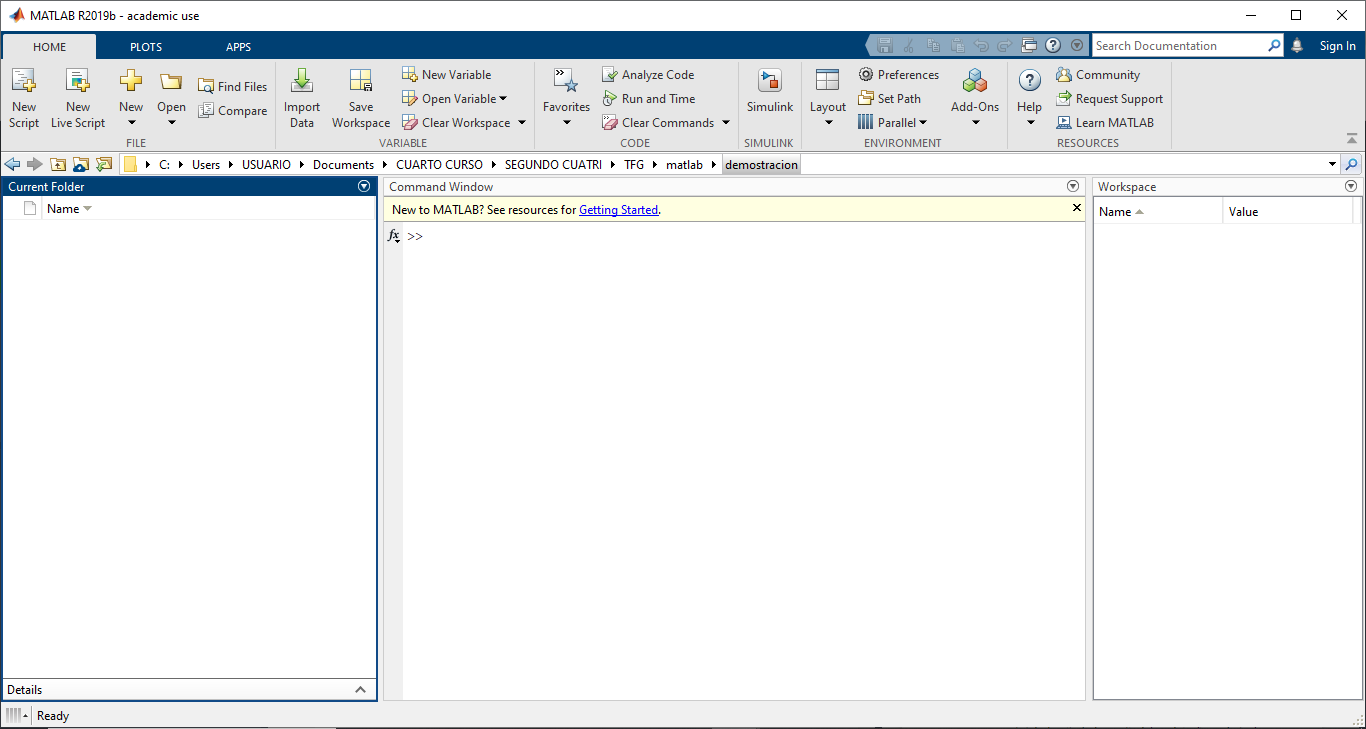
\includegraphics[width=1.1\linewidth]{img/anexos/manual/inicio.PNG}
    \caption{Página de inicio de MatLab.}
    \label{fig:inicio_matlab}
\end{figure}

Para crear o abrir scrips, en el \textbf{\textit{Panel HOME}} se pulsa \textit{New Script} (para crear nuevos) o bien \textit{Open} (para abrirlos desde una carpeta):
\clearpage

\begin{figure}[htbp]
    \centering
    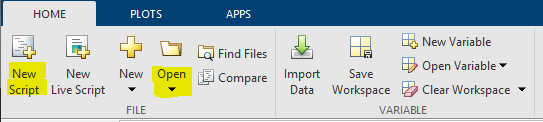
\includegraphics[width=0.8\linewidth]{img/anexos/manual/archivo.PNG}
    \caption{Crear un script en MatLab.}
    \label{fig:crear_script}
\end{figure}

Una vez abierto el script, como se muestra en, se prueba que al ejecutarlo mediante Run aparece la ejecución de dicho archivo en MatLab.

\begin{figure}[htbp]
    \centering
    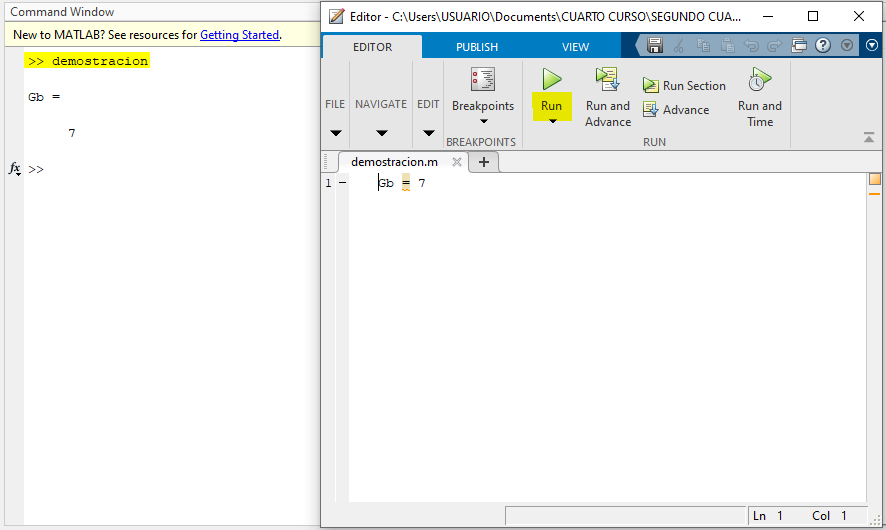
\includegraphics[width=0.8\linewidth]{img/anexos/manual/ej.PNG}
    \caption{Ejecución de un script en MatLab.}
    \label{fig:ejecutar_script}
\end{figure}

Para abrir Simulink, en el \textbf{\textit{Panel HOME}} se pulsa \textit{Simulink} (Figura \ref{fig:abrir_simulink}) y, una vez en la \textit{Simulink Start Page} se abre un \textit{"Blank Model"} (Figura \ref{fig:simulink}).

\begin{figure}[htbp]
    \centering
    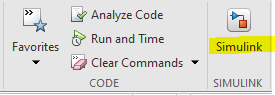
\includegraphics[width=0.5\linewidth]{img/anexos/manual/simulink.PNG}
    \caption{Abrir Simulink en MatLab.}
    \label{fig:abrir_simulink}
\end{figure}
\clearpage
\begin{figure}
    \centering
    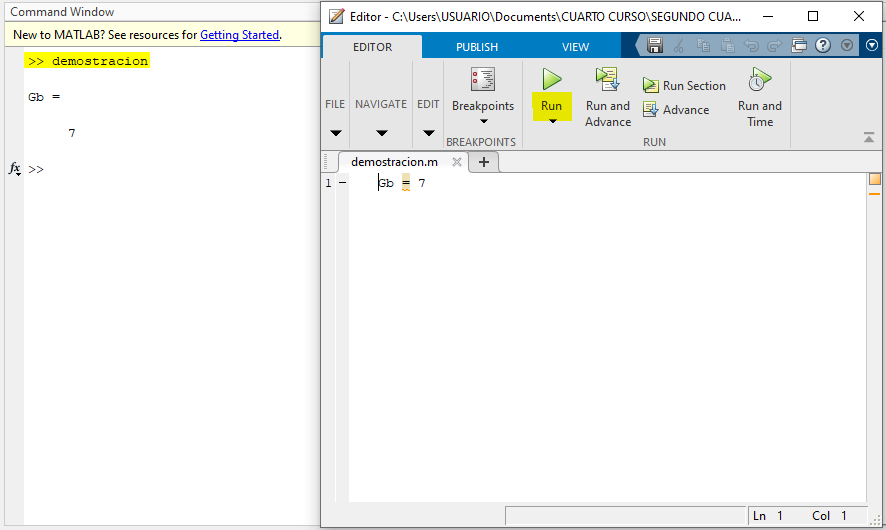
\includegraphics[width=1.1\linewidth]{img/anexos/manual/ej.PNG}
    \caption{Simulink Start Page.}
    \label{fig:simulink}
\end{figure}

Dentro de Simulink (Figura \ref{fig:inicio_simulink}) , se encuentra el marco de trabajo donde se ha realizado este estudio. La librería Simulink Library Browser de la Figura \ref{fig:library_simulink}, es una ventana dentro del entorno de Simulink que proporciona acceso a una amplia variedad de bloques predefinidos y funciones para construir modelos de simulación. 
\clearpage
\begin{figure}[htbp]
    \centering
    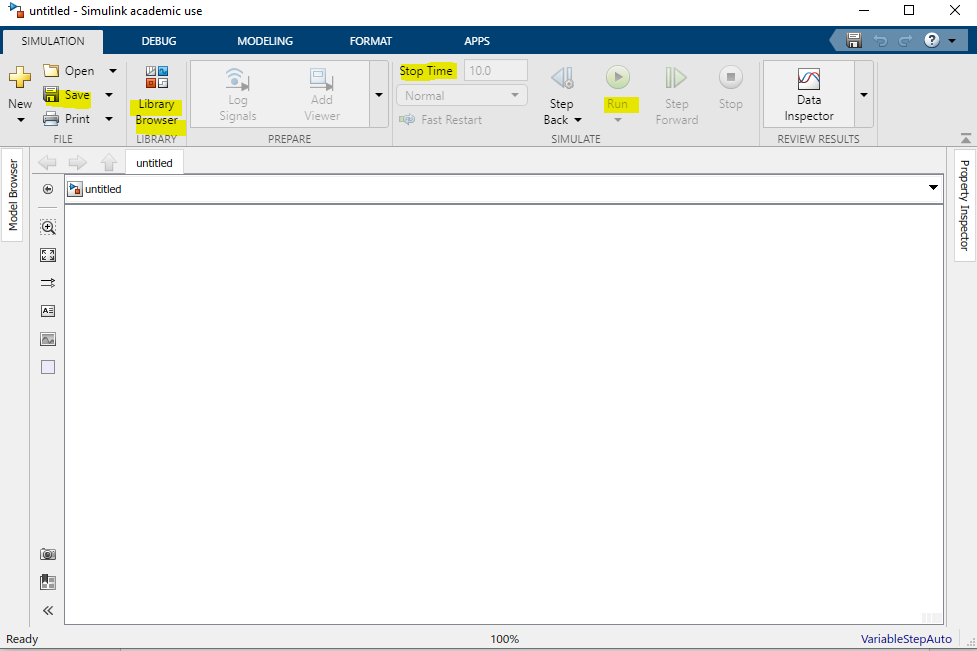
\includegraphics[width=1.1\linewidth]{img/anexos/manual/simulink_start.PNG}
    \caption{Página de inicio de Simulink.}
    \label{fig:inicio_simulink}
\end{figure}
\clearpage
\begin{figure}[htbp]
    \centering
    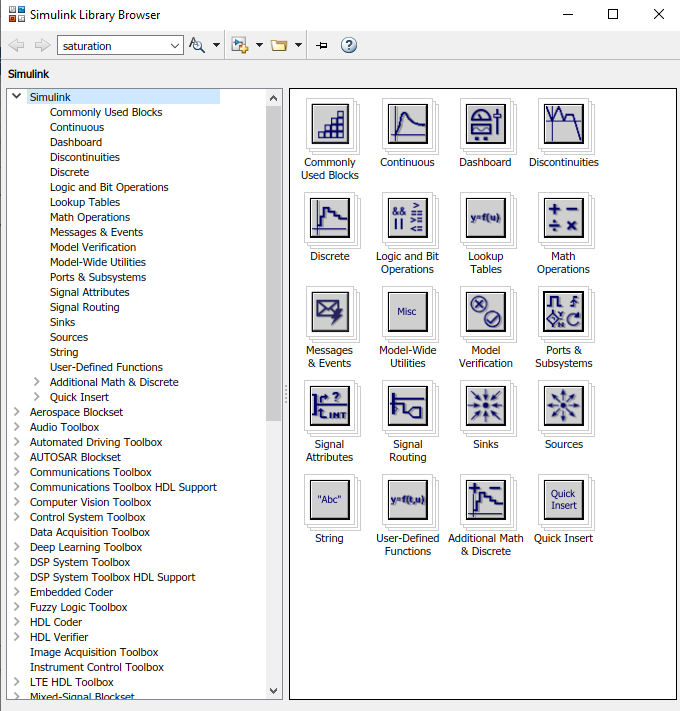
\includegraphics[width=0.9\linewidth]{img/anexos/manual/library.PNG}
    \caption{Simulink Library Browser.}
    \label{fig:library_simulink}
\end{figure}

Mediante \textit{"Stop Time"} se define la duración de la simulación a realizar en segundos, y mediante \textit{"Run"} se ejecuta la simulación. La inclusión de los bloques se realiza arrastrándoles hacia el marco de trabajo.

Se incluyen a continuación los bloques más relevantes para este proyecto:
\begin{enumerate}
    \item Bloques \textit{Sum, Substract, Product, Divide} para realizar operaciones matemáticas básicas.
     \item Bloque \textit{Integrador/Integrator}, para modelar las ecuaciones diferenciales de los modelos matemáticos.
     \item Bloques\textit{ Constant} y \textit{Gain}, para incluir parámetros constantes.
     \item Bloques \textit{Rampa/Ramp, Escalón/Step} para generar señales de entrada.
     \item Bloque\textit{ Scope}, para crea gráficas con las salidas resultantes.
\end{enumerate}

Para guardar los archivos basta con presionar \textit{CONTROL + S}.

Para más información consultar los tutoriales de MatLab en \cite{matlab_intro}.